\documentclass{article}
\usepackage{tikz}

\begin{document}

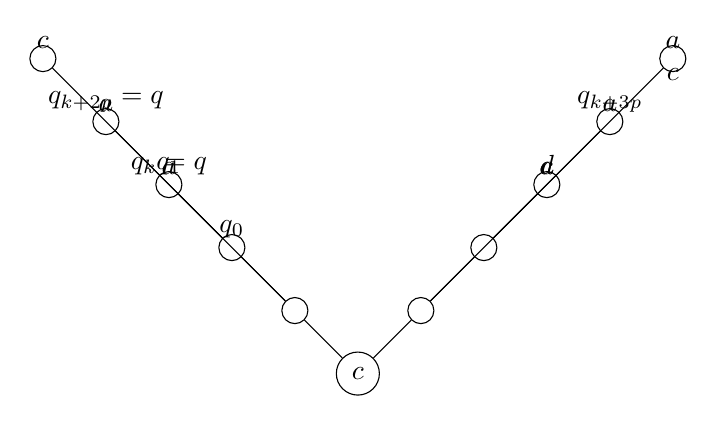
\begin{tikzpicture}[scale=0.8]
  \node (root) at (0,0) [circle,draw] {$c$};
  \node (child1) at (-1,1) [circle,draw] {};
  \node (child2) at (1,1) [circle,draw] {};
  \node (child3) at (-2,2) [circle,draw] {};
  \node (child4) at (-3,3) [circle,draw] {};
  \node (child5) at (2,2) [circle,draw] {};
  \node (child6) at (3,3) [circle,draw] {};
  \node (child7) at (-4,4) [circle,draw] {};
  \node (child8) at (-5,5) [circle,draw] {};
  \node (child9) at (4,4) [circle,draw] {};
  \node (child10) at (5,5) [circle,draw] {};

  \draw (root) -- (child1);
  \draw (root) -- (child2);
  \draw (child1) -- (child3);
  \draw (child1) -- (child4);
  \draw (child2) -- (child5);
  \draw (child2) -- (child6);
  \draw (child3) -- (child7);
  \draw (child3) -- (child8);
  \draw (child5) -- (child9);
  \draw (child5) -- (child10);

  \path (child7) node [above] {$q_{k+2p}=q$};
  \path (child9) node [above] {$q_{k+3p}$};
  \path (child8) node [above] {$c$};
  \path (child10) node [below] {$c$};

  \path (child4) node [above] {$q_k=q$};
  \path (child6) node [above] {$d$};
  \path (child4) node [above] {$q_1$};
  \path (child6) node [above] {$c$};
  \path (child3) node [above] {$q_0$};
  \path (child4) node [above] {$a$};
  \path (child6) node [above] {$a$};
  \path (child10) node [above] {$a$};
  \path (child7) node [above] {$a$};
  \path (child9) node [above] {$a$};
\end{tikzpicture}

\end{document}